\chapter{Risultati sperimentali} % (fold)
\label{chap:Risultati sperimentali}

\section{Addestramento} % (fold)
\label{sec:Addestramento}

Il modello \`e stato addestrato mediante l'uso della \textit{cross-validation}(\autoref{fig:cross_validation})
con una suddivisione dei dati in 5 parti uguali(5 folds).

Essendo una tipologia di apprendimento supervisionata, al modello sono fornite immagini
originali e le loro segmentazioni effettuate manualemte.

\begin{figure}[!ht]
	\begin{adjustbox}{width=0.7\columnwidth, center}
    \includegraphics{./images/training.png}
  \end{adjustbox}
  \caption{Addestramento del modello}
  \label{fig:addestramento del modello}
\end{figure}

Effettuando l'addestramento con 5 folds, il modello viene addestrato 5 volte, ogni volta con un fold diverso,
l'errore finale \`e dato dalla media degli errori ottenuti dalle 5 iterazioni.

\begin{figure}[!ht]
	\begin{adjustbox}{width=0.9\columnwidth, center}
    \includegraphics{./images/fold_0_loss.png} \includegraphics{./images/fold_0_accuracy.png}
  \end{adjustbox}
  \caption{Errore e accuratezza della prima porzione di dati}
  \label{fig:loss e accuratezza della prima porzione di dati}
\end{figure}

\begin{figure}[!ht]
	\begin{adjustbox}{width=0.9\columnwidth, center}
    \includegraphics{./images/fold_1_loss.png} \includegraphics{./images/fold_1_accuracy.png}
  \end{adjustbox}
  \caption{Errore e accuratezza della seconda porzione di dati}
  \label{fig:loss e accuratezza della seconda porzione di dati}
\end{figure}

\begin{figure}[!ht]
	\begin{adjustbox}{width=0.9\columnwidth, center}
    \includegraphics{./images/fold_2_loss.png} \includegraphics{./images/fold_2_accuracy.png}
  \end{adjustbox}
  \caption{Errore e accuratezza della terza porzione di dati}
  \label{fig:loss e accuratezza della terza porzione di dati}
\end{figure}

\begin{figure}[!ht]
	\begin{adjustbox}{width=0.9\columnwidth, center}
    \includegraphics{./images/fold_3_loss.png} \includegraphics{./images/fold_3_accuracy.png}
  \end{adjustbox}
  \caption{Errore e accuratezza della quarta porzione di dati}
  \label{fig:loss e accuratezza della quarta porzione di dati}
\end{figure}

\begin{figure}[!ht]
	\begin{adjustbox}{width=0.9\columnwidth, center}
    \includegraphics{./images/fold_4_loss.png} \includegraphics{./images/fold_4_accuracy.png}
  \end{adjustbox}
  \caption{Errore e accuratezza della quinta porzione di dati}
  \label{fig:loss e accuratezza della quinta porzione di dati}
\end{figure}

L'\textbf{errore} medio del modello \`e di \textbf{$8\%$} mentre l'\textbf{accuratezza} media \`e di \textbf{$92\%$}(le metriche utilizzate \autoref{sec:metriche}).



Considerando che questo modello \`e stato utilizzato in ambito medico per velocizzare e standardizzare 
la segmentazione dei femori per un'analisi su questi ultimi, oltre ad analisi quantitative, \`e stato 
necessario effettuare delle analisi qualitative sulal segmentazione ottenuta dal modello.

Nelle immagini seguenti viene riportato uno delle immagini prese in considerazione per l'addestramento del modello
e vengono mostrate le segmentazione manuali, le segmentazioni ottenute dal modello e la differenze 
nella classificazione dei pixel tra le due segmentazioni.


Partendo da una immagini (\autoref{fig:immagine originale}) ottenuta mediante la raccolta dati effettuata dai medici, 

\begin{figure}[!ht]
	\begin{adjustbox}{width=0.8\columnwidth, center}
    \includegraphics{./images/image.png}
  \end{adjustbox}
  \caption{Immagine originale}
  \label{fig:immagine originale}
\end{figure}

I risultati ottenuti mediante la segmentazione manuale e la segmentazione del modello sono i seguenti:
\begin{figure}[!ht]
	\begin{adjustbox}{width=0.9\columnwidth, center}
    \includegraphics{./images/mask.png}
    \hspace{20pt} % Add horizontal space between the two images
    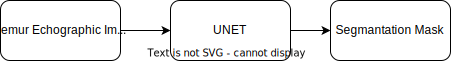
\includegraphics{./images/prediction.png}
  \end{adjustbox}
  \caption{Segmentazione manuale(sinistra) e segmentazione del modello(destra)}
  \label{fig:segmentazione manuale e segmentazione del modello}
\end{figure}


Per sostenere la tesi che il modello riesca a segmentare correttamente le immagini, \`e stata 
calcolata la distribuzione dei pixel per controntare la segmentazione manuale con quella del modello.

\begin{figure}[!ht]
	\begin{adjustbox}{width=0.9\columnwidth, center}
    \includegraphics{./images/handmade_scaled_hist.png}
    \hspace{20pt} % Add horizontal space between the two images
    \includegraphics{./images/model_scaled_hist.png}
  \end{adjustbox}
  \caption{Distribuzione dei pixel della segmentazione manuale(sinistra) e del modello(destra)}
  \label{fig:distribuzione dei pixel della segmentazione manuale e del modello}
\end{figure}

Un'altra rappresentazione a confronto dei risultati ottenuti \`e la seguente:

\begin{figure}[!ht]
	\begin{adjustbox}{width=0.8\columnwidth, center}
    \includegraphics{./images/handmade_vs_model_scaled.png}
  \end{adjustbox}
  \caption{Confronto tra la segmentazione manuale e quella del modello}
  \label{fig:confronto tra la segmentazione manuale e quella del modello}
\end{figure}

Dai risultati qualitatitivi e quantitativi si pu\`o constatare che il modello ha una performance
molto promettente in quanto supera abbondantemente un'accuratezza del $90\%$ e pu\`o essere 
addestrato incrementando il numero di imamgini a disposizione. 

Non sono necessari ulteriori segmentazioni manuali ma si possono direttamente sfruttare
le nuove immagini raccolte, segmentarle mediante l'uso del modello e utilizzarle per l'addestramento.




% section Addestramento (end)

\section{Problema} % (fold)
\label{sec:Problema}



% Prenatal estimation/quantification of the bone mineral density of the fetal femur by means of an artificial intelligence-based algorithm and relationship with birthweight: preliminary results from a pilot study. 
%
%  
%
% Authors: 
%
% Dall’Asta, Ferrari, Ollari Ischimji, Celora, Degennaro, Prati, Ghi 
%
%  
%
% Objective 
%
% To evaluate the relationship between the bone mineral density (BMD) of the fetal femur estimated/quantified by means of an artificial intelligence-based algorithm and the birthweight. 
%
%  
%
% Methods 
%
% Single center prospective study conducted at a tertiary maternity unit in Italy between April 2022 and January 2023 and including a selected cohort of women submitted to prenatal assessment with between 35+0 and 37+0 weeks. Only singleton pregnancies from women of Caucasian ethnicity and booking BMI between 20 and 25 were included. In such cases a standard image of the fetal femur was acquired using one single US machine and offline processed using an artificial intelligence-based algorithm allowing the automated quantification of the pixels contained in the femoral area together with their relative brightness to estimate the BMD of the fetal femur, which was correlated with the birthweight percentile. 
%
%  
%
% Results 
%
% Overall, 151 cases meeting the inclusion criteria were included at a median gestation of 36+2 (35+0-37+0) weeks, of whom 27 (17.9%) had a postnatal diagnosis of SGA. No correlation was found between estimated BMD and birthweight percentile (Pearson’s correlation 0.064, p=0.433), however a trend towards increasing birthweight with increasing brightness of the fetal femur was noted (Figure 1). Cases with a postnatal diagnosis of SGA showed a non-significantly lower mean BMD compared to AGA fetuses (144.6+22.4 vs 148.7+21.3, p=0.36). 
%
%  
%
% Conclusions 
%
% Though no significant correlation was found between bone mineral density and birth weight centile, a trend towards a lower BMD with decreasing birthweight percentile was noted. The relationship between birthweight and estimated BMD warrants further investigation from prospective data.  





% WARN: SECOND STUDY
% Development of an artificial intelligence-based algorithm for the prenatal estimation/quantification of the fetal bone mineral density. 
%
%  
%
% Authors: 
%
% Dall’Asta, Ferrari, Ollari Ischimji, Celora, Degennaro, Prati, Ghi 
%
%  
%
% Objective 
%
% To report the development of an artificial intelligence-based algorithm for the prenatal quantification of the fetal bone mineral density (BMD). 
%
%  
%
% Methods 
%
% Single center prospective study conducted at a tertiary maternity unit in Italy between April 2022 and January 2023 and including a selected cohort of women submitted to prenatal assessment with between 35+0 and 37+0 weeks. Only singleton pregnancies from women of Caucasian ethnicity and booking BMI between 20 and 25 were included. The collected data include standard images of the fetal femur acquired with one single US machine, which were manually processed by a single operator to obtain the segmentation of the fetal femur contour i.e., the spatial location of the femur in the US image. These data represent the gold standard reference and were subsequently used to train a deep neural network to perform the segmentation of the fetal femoral area automatically. Both manual and neural network-derived segmentations are then used to isolate the fetal femur region from the US image, allowing the automated quantification of the pixels contained in the femoral area together with their relative brightness, the latter being hypothesized to be correlated with the BMD of the fetal femur. 
%
%  
%
% Results 
%
% Overall, 151 cases meeting the inclusion criteria were considered at a median gestation of 36+2 (35+0-37+0) weeks. The gold standard and the artificial intelligence-based segmentations showed a 92% agreement in the quantification and detection of the pixels contained in the femoral area and their relative brightness, evidencing the output of the neural network is reliable to be used for subsequent analyses. We observed the relative brightness being normally distributed, from which reference ranges for the gestation were obtained (table 1). 
%
%  
%
% Conclusions 
%
% An algorithm for the automated segmentation of the fetal femoral area and reference ranges of proportionate pixel brightness were developed. This could assist in correlating the brightness of the femoral area with bone mineral density in cases at low- and high- risk for demineralization of the fetal bone. 
%
%

% section Problema (end)




% chapter Risultati sperimentali (end)
